\documentclass[10pt]{article}

\usepackage[margin=0.75in]{geometry}
\usepackage{amsmath,amsthm,amssymb}
\usepackage{xcolor}
\usepackage{cancel}
\usepackage{graphicx}
\usepackage{changepage}
\usepackage{circuitikz}
\usepackage{pgfplots}
\usepackage{physics}
\usepackage{hyperref}
\usepackage{siunitx}
\usepackage{fontspec}
\usepackage{relsize}
\usepackage{subfig}
\usepackage{todonotes}
\usepackage{multicol, multirow, booktabs}
\usepackage[breakable]{tcolorbox}
\usepackage[inline]{enumitem}

\theoremstyle{definition}
\newtheorem{problem}{Problem}
\newtheorem{soln}{Solution}

\pgfplotsset{compat=newest}
\usetikzlibrary{lindenmayersystems}
\usetikzlibrary{arrows}
\usetikzlibrary{calc}
\usetikzlibrary{positioning, fit}
\usetikzlibrary{3d, perspective}

\definecolor{incolor}{HTML}{303F9F}
\definecolor{outcolor}{HTML}{D84315}
\definecolor{cellborder}{HTML}{CFCFCF}
\definecolor{cellbackground}{HTML}{F7F7F7}
\newcommand{\ui}{\hat{i}}
\newcommand{\uj}{\hat{j}}
\newcommand{\uk}{\hat{k}}
\newcommand{\ux}{\hat{x}}
\newcommand{\uy}{\hat{y}}
\newcommand{\uz}{\hat{z}}
\newcommand{\primed}[1]{#1^\prime}
\pgfdeclarelayer{background}  
\pgfsetlayers{background,main}
\AtBeginDocument{\RenewCommandCopy\qty\SI}

\makeatletter
\newcommand{\boxspacing}{\kern\kvtcb@left@rule\kern\kvtcb@boxsep}
\makeatother
\newcommand{\prompt}[4]{
    \ttfamily\llap{{\color{#2}[#3]:\hspace{3pt}#4}}\vspace{-\baselineskip}
}

\newcommand{\thevenin}[2]{
  \begin{center}
    \begin{circuitikz} \draw
      (0,0) -- (2,0) to[battery1, l_=$V_{Th}\eq#1$] (2,2) 
      to[resistor, l_=$R_{Th}\eq#2$] (0,2)
      ;
      \draw [o-] (-.07,2.079);
      \draw [o-] (-.07,0.079);
    \end{circuitikz}
  \end{center}
}

\newcommand{\norton}[2]{
  \begin{center}
    \begin{circuitikz} \draw
      (0,0) -- (3,0) to[american current source, l_=$I_{N}\eq#1$] (3,2) -- (0,2) (2,0)
      to[resistor, l=$R_{N}\eq#2$] (2,2)
      ;
      \draw [o-] (-.07,2.079);
      \draw [o-] (-.07,0.079);
    \end{circuitikz}
  \end{center}
}

\newcommand{\highlight}[1]{\colorbox{yellow}{$\displaystyle #1$}}

\newcommand{\ti}[1]{\widetilde{#1}}

\newfontface{\Kaufmann}{Kaufmann}
\DeclareTextFontCommand{\kf}{\Kaufmann}
\newcommand{\scriptr}{\fontsize{12pt}{12pt}\kf{r}}

\newfontface{\KaufmannB}{Kaufmann Bd BT}
\DeclareTextFontCommand{\kfb}{\KaufmannB}
\newcommand{\bscriptr}{\fontsize{12pt}{12pt}\kfb{r}}

\newcommand{\bv}[1]{\mathbf{#1}}

\title{Physics 3610H: Assignment II}
\author{Jeremy Favro (0805980) \\ Trent University, Peterborough, ON, Canada}
\date{\today}

\begin{document}
\maketitle

% PROBLEM 1
\begin{problem} Consider a single particle of mass m moving in one dimension subject to the following
potential:
$$
  V(x)=\begin{cases}
    \infty, & x<-c   \\
    0,      & -c<x<c \\
    \infty, & x>c
  \end{cases}
$$
\begin{enumerate}[label=(\alph*)]
  \item Find the eigenvalues and eigenstates of $\hat{H}$ for this system, that is the energies $E$ and the
        states $\psi$ for which $\hat{H}\psi=E\psi$.
  \item Examine the two lowest energy states:
        \begin{enumerate}[label=(\roman*)]
          \item Draw two plots showing $\psi$ vs $x$ for the two lowest energy states.
          \item This is very similar to the problem we solved in class. Comment on whether your results
                for the two lowest energy states (both the energies and the states) are consistent with those
                we found in class.
          \item Show that the two lowest energy states are orthogonal.
        \end{enumerate}
\end{enumerate}
\end{problem}
\begin{soln}~
  \begin{enumerate}[label=(\alph*)]
    \item Here $\hat{H}$ is the operator corresponding to the total energy of the particle. Because the particle is only subject to the potential
          applied by the well at its edges and possesses only kinetic energy otherwise we can say
          $$\hat{H}=-\frac{\hbar^2}{2m}\frac{\partial}{\partial x} + V(x)$$
          where we've obtained the operator corresponding to kinetic energy by using the momentum operator in the usual expression for kinetic energy.
          Now that we have $\hat{H}$ we can solve the time dependent Schr\"odinger equation,
          $$i\hbar\frac{\partial}{\partial t}\Psi(x,t)=\hat{H}\Psi(x,t)$$
          which, when we substitute our $\hat{H}$ becomes
          $$i\hbar\frac{\partial}{\partial t}\Psi(x,t)=\left[-\frac{\hbar^2}{2m}\frac{\partial^2}{\partial x^2} + V(x)\right]\Psi(x,t).$$
          We will try now to find a $\Psi(x,t)$ which is separable as $\Psi(x,t)=\psi(x)\phi(t)$ this doesn't always work but from some foreknowledge
          of the problem we know there is a fair chance that it will and so we try it. This means that our equation is now
          $$i\hbar\frac{\partial}{\partial t}\psi(x)\phi(t)=\left[-\frac{\hbar^2}{2m}\frac{\partial^2}{\partial x^2}  + V(x)\right]\psi(x)\phi(t).$$
          We can divide through on both sides by $\psi(x)\phi(t)$ being careful to note that we cannot pull functions out of derivatives that contain
          the variable of differentiation, e.g. on the left side $\phi$ will not cancel and the derivative will instead be multiplied out front
          by $\phi^{-1}$. This makes our equation now
          $$\frac{i\hbar}{\phi(t)}\frac{\partial}{\partial t}\phi(t)=\frac{1}{\psi(x)}\left[-\frac{\hbar^2}{2m}\frac{\partial^2}{\partial x^2}  + V(x)\right]\psi(x)$$
          which satisfies our original reason for trying to separate $\Psi$: to obtain two differential equations of only on variable each which makes them ODEs instead
          of PDEs. Another consequence of this separation while maintaining equality is that these functions must \emph{always} be equal. The only way this can happen
          is if both are equal to a constant as fixing one variable and varying the other would (if they were not equal to a constant), to preserve equality, require that $x$ and $t$
          are related in a way that makes this possible. This is obviously not the case so we can reason that regardless of values of $x$ or $t$, the two must be the same and constant.
          This allows us to further ``separate'' the equation into two independent ODEs,
          \begin{align}
            E & =\frac{i\hbar}{\phi(t)}\frac{d}{d t}\phi(t) \label{eq1}                                      \\
            E & =\frac{1}{\psi(x)}\left[-\frac{\hbar^2}{2m}\frac{d^2}{d x^2} + V(x)\right]\psi(x)\label{eq2}
          \end{align}
          We will first begin by solving \ref{eq1} as it is very easy by recognizing that there is an easy function whose derivative is itself times a constant, $e^x$.
          This gives us
          $$\phi=Ce^{-iEt/\hbar}$$
          where $C$ is a constant of integration.
          Now for \ref{eq2} with some rearranging (and noticing the $V(x)=0$ in the region we care about) we have
          $$-\frac{2mE}{\hbar^2}\psi(x)=\frac{d^2}{d x^2}\psi(x).$$
          This means we are looking now for a function whose second derivative is itself times a negative constant.
          This is satisfied by
          $$\psi(x)=A\sin\left(kx\right)+B\cos\left(kx\right).$$
          where $k=\sqrt{\frac{2mE}{\hbar^2}}$.
          We can now work to determine $k$ (really $E$) using the implied boundary conditions given by the fact that the particle may not exist at $x=\pm c$ 
          as it would require a nonphysical energy, meaning the wavefunction
          must be zero there. Applying this gives
          $$\psi(c)=A\sin\left(kc\right)+B\cos\left(kc\right)=0$$
          and
          $$\psi(-c)=A\sin\left(-kc\right)+B\cos\left(-kc\right)=-A\sin\left(kc\right)+B\cos\left(kc\right)=0.$$
          The fact that both of these are zero is satisfied only by
          $$A\sin\left(kc\right)=B\cos\left(kc\right)=0.$$
          The only way this can happen is if either $A=B=0$ meaning the probability of the particle being found anywhere is zero and the particle therefore does not exist
          or the more useful case of $k$ being some value that makes either $\sin\left(kc\right)$ or $\cos\left(kc\right)$ zero. Knowing that
          $k$ must be the same for both functions this gives rise to two possible solutions. For $\sin(x)$ to be zero $x$ must be some integer multiple of $\pi$ and
          for $\cos(x)$ to be zero $x$ must be some \emph{half} integer multiple of $\pi$. The only way to satisfy this is to construct a $k$ of the form
          $$k=\frac{n\pi}{2c}$$
          and use the $\sin(kx)$ function for even values of $n$ and $\cos(kx)$ for odd values. It's also important to note that we require $n\in \mathbb{Z}>0$
          as the negative $n$s are just multiples of the positive ones (due to the odd/even nature of our trig functions) and so give no new information and $n=0$ is again the no-particle-exists case
          and also gives no information. So we now have two possible functions for $\psi_n(x)$,
          $$
            \psi_n(x) =
            \begin{cases}
              A\sin(kx),\qquad n=2,4,6,\dots \\
              B\cos(kx),\qquad n=1,3,5,\dots \\
            \end{cases}
          $$
          Working out $E$ now as it is the only thing inside $k$ which we can set to force $k$ to adopt our constructed value,
          \begin{align*}
            k        & =\frac{n\pi}{2c}=\sqrt{\frac{2mE}{\hbar^2}} \\
            \implies & \frac{n^2\pi^2}{4c^2}=\frac{2mE}{\hbar^2}   \\
            \implies & \frac{n^2\pi^2\hbar^2}{8mc^2}=E_n
          \end{align*}
          Now using our last available bit of information, the requirement that the probability of finding the particle anywhere must be 1,
          we integrate our wavefunction (either one! both have the same amplitude and will therefore have the same constant) over all space and force it to be 1 using the constants.
          We can also note that helpfully the particle is guaranteed to only exist within the well so we can narrow down our bounds of integration,
          \begin{align*}
            1 & =\int_{-c}^{c}\psi(x)\psi^*(x)dx                                                                                 \\
              & =\int_{-c}^{c}\left|A\right|\sin\left(\frac{n\pi}{2c}x\right)\left|A\right|\sin\left(\frac{n\pi}{2c}x\right)\,dx \\
              & =\left|A\right|^2\int_{-c}^{c}\sin^2\left(\frac{n\pi}{2c}x\right)\,dx                                            \\
              & =\frac{\left|A\right|^2}{2}\left[\int_{-c}^{c}1\,dx-\int_{-c}^{c}\cos\left(\frac{n\pi}{c}x\right)\,dx\right]     \\
              & =\frac{\left|A\right|^2}{2}\left[2c-\int_{-c}^{c}\cos\left(\frac{n\pi}{c}x\right)\,dx\right]                     \\
              & =\frac{\left|A\right|^2}{2}\left[2c-\frac{2c}{n\pi}\cancelto{0}{\sin(\pi n)}\right]
              & \implies c \left|A\right|^2=1\implies \left|A\right|=\sqrt{\frac{1}{c}}
          \end{align*}
          By example of the text we pick the positive real value of $\left|A\right|$ and so obtain
          $$
            \psi_n(x) =
            \begin{cases}
              \sqrt{\frac{1}{c}}\sin(\frac{n\pi}{2c}x),\qquad n=2,4,6,\dots \\
              \sqrt{\frac{1}{c}}\cos(\frac{n\pi}{2c}x),\qquad n=1,3,5,\dots \\
            \end{cases}
          $$
          We can now say that the above $\psi_n(x)$s are our eigenstates and $E_n=\displaystyle\frac{n^2\pi^2\hbar^2}{8mc^2}$ our eigenvalues.
          \newpage
    \item ~\\
          \begin{enumerate}[label=(\roman*)]
            \item ~\\ \begin{center}
                    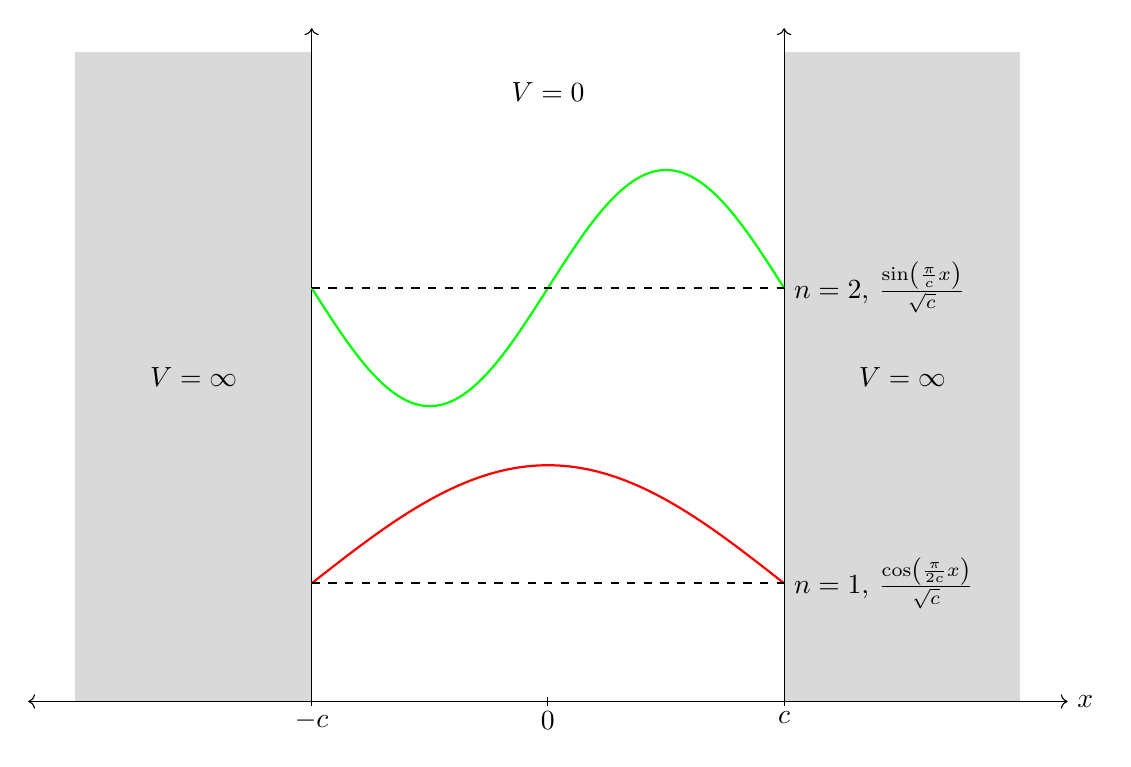
\begin{tikzpicture}[x=2cm, scale=1.5]
                      \def\topval{5.5}
                      \fill[gray!30]
                      (-1, 0) rectangle (-2, \topval);
                      \fill[gray!30]
                      (1, 0) rectangle (2, \topval);
                      \node at (-1.5, \topval/2) { $V = \infty$};
                      \node at (1.5, \topval/2) {$V = \infty$};

                      \node[anchor = north] at (-1, 0)   { $-c$};
                      \node[anchor = north] at (0, 0)   {0};
                      \node[anchor = north] at (1, 0)   {$c$};
                      \node[anchor = west] at (2.2, 0)   {$x$};
                      \node[anchor = south] at (0, \topval-0.5) { $V = 0$};
                      \draw[<->] (-2.2, 0) to (2.2, 0);
                      \draw[] (0,-0.04) -- (0,0.04);
                      \draw[->]  (1, -0.04) to (1, \topval+0.2);
                      \draw[->]  (-1, -0.04) to (-1, \topval+0.2);


                      \draw[red, thick, domain=-1:1, samples=100] plot (\x, {cos(deg(pi*\x/2))+1}) node[right, black] {$n=1$, $\frac{\cos(\frac{\pi}{2c}x)}{\sqrt{c}}$};
                      \draw[dashed, thick] (-1,1) --(1,1);
                      \draw[green, thick, domain=-1:1, samples=100] plot (\x, {sin(deg(pi*\x))+3.5}) node[right, black] {$n=2$, $\frac{\sin(\frac{\pi}{c}x)}{\sqrt{c}}$};
                      \draw[dashed, thick] (-1,3.5) --(1,3.5);
                      % \draw[blue, thick, domain=0:4, samples=200] plot (\x, {sin(360*\x/4)}) ;
                      % \draw[green, thick, domain=0:4, samples=200] plot (\x, {sin(540*\x/4)})  ;
                    \end{tikzpicture}
                  \end{center}
            \item Yes, the results obtained here are consistent with those in class. In class we had a well with width $a$ and here we have a well with width
                  $2c$. This means we'd see a doubling everywhere there is width dependent term.
                  For the energy eigenvalues acting as if we are now in a well of half the width we obtain $\displaystyle\frac{n^2\pi^2\hbar^2}{8m(c/2)^2}=\frac{n^2\pi^2\hbar^2}{2mc^2}$
                  which is the same as what we obtained in class. For the eigenstates we see
                  $$
                    \psi_n(x) =
                    \begin{cases}
                      \sqrt{\frac{1}{c/2}}\sin(\frac{n\pi}{2(c/2)}x),\qquad n=2,4,6,\dots \\
                      \sqrt{\frac{1}{c/2}}\cos(\frac{n\pi}{2(c/2)}x),\qquad n=1,3,5,\dots \\
                    \end{cases}
                  $$
                  Which simplifies down to
                  $$
                    \psi_n(x) =
                    \begin{cases}
                      \sqrt{\frac{2}{c}}\sin(\frac{n\pi}{c}x),\qquad n=2,4,6,\dots \\
                      \sqrt{\frac{2}{c}}\cos(\frac{n\pi}{c}x),\qquad n=1,3,5,\dots \\
                    \end{cases}
                  $$
                  which is similar to what we had in class, the only difference coming from the fact that we have assumed that the origin is in the middle of our bounds.
                  If we followed the previous math used to obtain these $\psi$ values but assumed the origin was at the left bound of a well with width $c/2$ we would obtain the in class
                  solution as we would expect.
            \item Orthogonality on functions is defined using the inner product of functions,
                  $$\int_{-c}^c f(x)g(x)\,dx$$
                  with the typical definition of orthogonality (0 means orthogonal). So,
                  \begin{align*}
                     & =\int_{-c}^c\psi_1(x)\psi_2(x)\,dx \\
                     & =\int_{-c}^c\sqrt{\frac{1}{c}}\cos(\frac{\pi}{2c}x)\sqrt{\frac{1}{c}}\sin(\frac{\pi}{c}x)\,dx \\
                     & =c^{-1}\int_{-c}^c\cos(\frac{\pi}{2c}x)\sin(\frac{\pi}{c}x)\,dx\rightsquigarrow u=\frac{\pi}{2c}x\implies du=\frac{\pi}{2c}dx\\
                     & =\frac{2}{\pi}\int_{-c}^c\cos(u)\sin(2u)\,du\rightsquigarrow \sin(2u)=2\sin (u)\cos (u)\\
                     & =\frac{2}{\pi}\int_{-c}^c2\cos^2(u)\sin(u)\,du\rightsquigarrow s=\cos(u)\implies ds=-\sin(u)du\\
                     & =-\frac{4}{\pi}\int_{-c}^cs^2\,ds\\
                     & =-\frac{4}{3\pi}\eval{s^3}_{-c}^{c}=-\frac{4}{3\pi}\eval{\cos^3(u)}_{-c}^{c}=-\frac{4}{3\pi}\eval{\cos^3\left(\frac{\pi}{2c}x\right)}_{-c}^{c}\\
                     & =-\frac{4}{3\pi}\left[\cos^3\left(\frac{\pi}{2c}c\right)-\cos^3\left(-\frac{\pi}{2c}c\right)\right]=0\\
                  \end{align*}
          \end{enumerate}
  \end{enumerate}
\end{soln}
\end{document}